\documentclass[12pt,fleqn]{article}\usepackage{../../common}
\begin{document}
M��teri Sadakatini Tahmin Etmek (Churn Prediction)

\inputminted[fontsize=\footnotesize]{python}{model.py}

\begin{minted}[fontsize=\footnotesize]{python}
import model

train_x = np.load("./data/train_x.npy")
train_y = np.load("./data/train_y.npy")
test_x = np.load("./data/test_x.npy")
test_y = np.load("./data/test_y.npy")

m = model.get_model()
m.load_weights('wtte.h5')
\end{minted}

\begin{minted}[fontsize=\footnotesize]{python}
# Make some predictions and put them alongside the real TTE and event
# indicator values
test_predict = m.predict(test_x)
test_predict = np.resize(test_predict, (100, 2))
test_result = np.concatenate((test_y, test_predict), axis=1)

# TTE, Event Indicator, Alpha, Beta
print(test_result[:10])
\end{minted}

\begin{verbatim}
[[ 112.            1.          199.97093201    3.82868171]
 [  98.            1.          180.49946594    3.690907  ]
 [  69.            1.           81.04798889    1.45907807]
 [  82.            1.           82.94621277    1.49614   ]
 [  91.            1.           86.75234985    1.57983696]
 [  93.            1.           82.14154816    1.49072194]
 [  91.            1.           81.48047638    1.47451472]
 [  95.            1.           82.19529724    1.49306989]
 [ 111.            1.          175.48095703    3.63983274]
 [  96.            1.           82.51445007    1.48723483]]
\end{verbatim}

[devam edecek]


\fbox{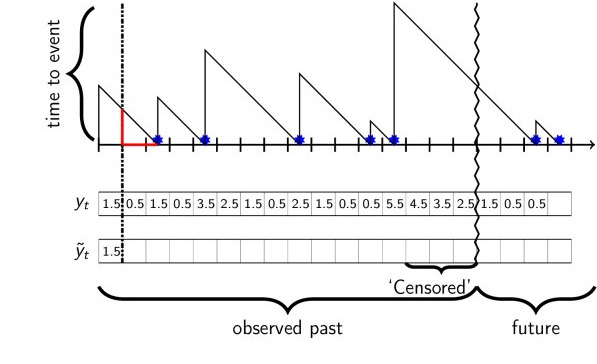
\includegraphics[width=20em]{censor-0.jpg}}
\fbox{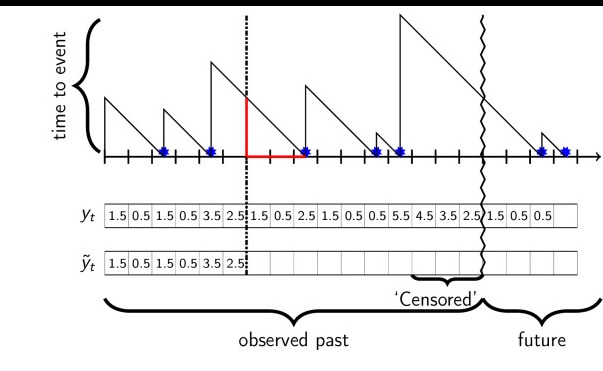
\includegraphics[width=20em]{censor-5.jpg}}

\fbox{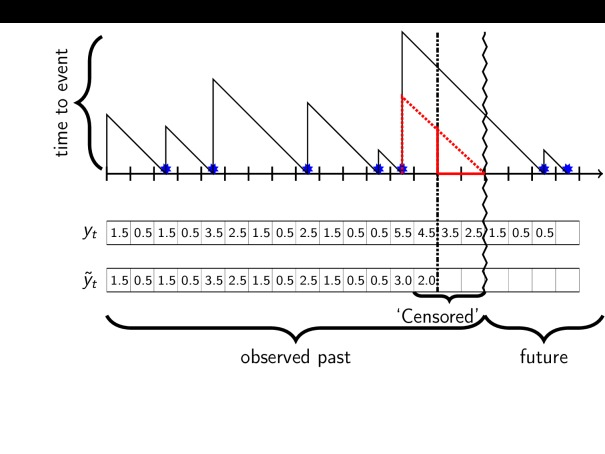
\includegraphics[width=20em]{censor-13.jpg}}
\fbox{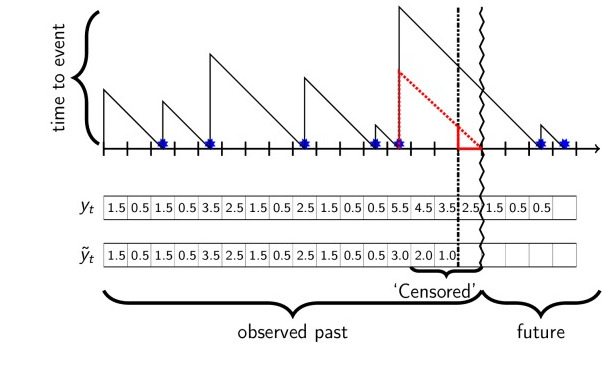
\includegraphics[width=20em]{censor-14.jpg}}

\fbox{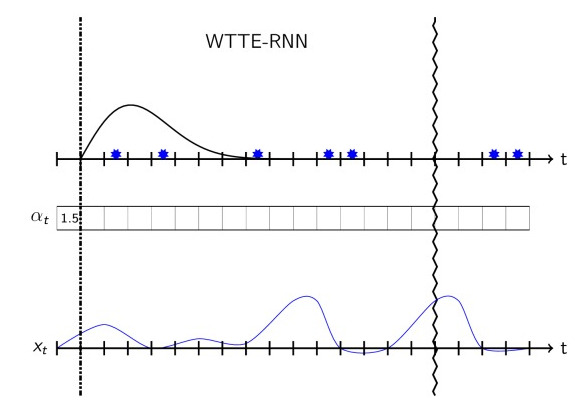
\includegraphics[width=20em]{wtte-0.jpg}}
\fbox{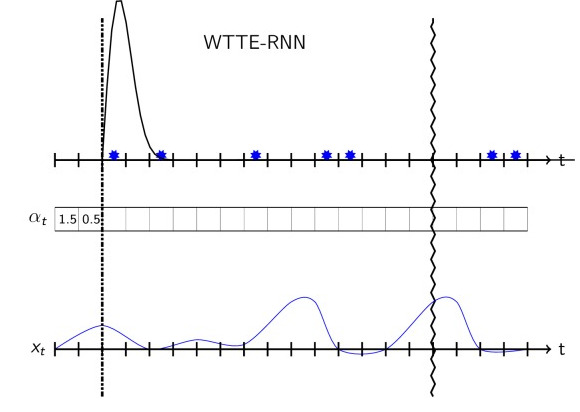
\includegraphics[width=20em]{wtte-1.jpg}}

\fbox{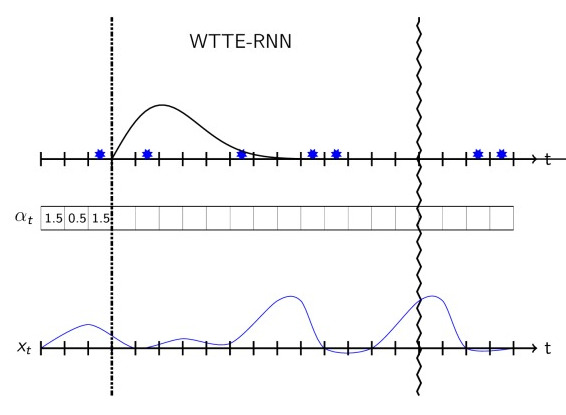
\includegraphics[width=20em]{wtte-2.jpg}}
\fbox{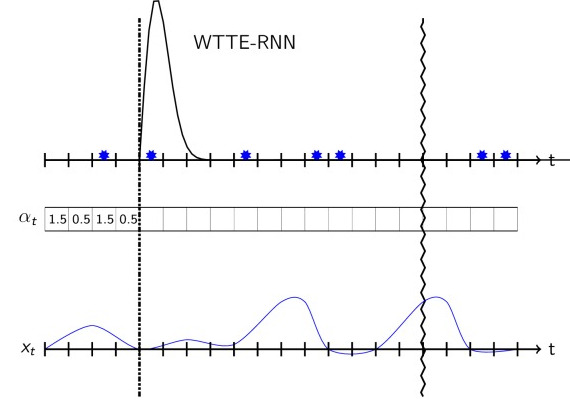
\includegraphics[width=20.5em]{wtte-3.jpg}}

\fbox{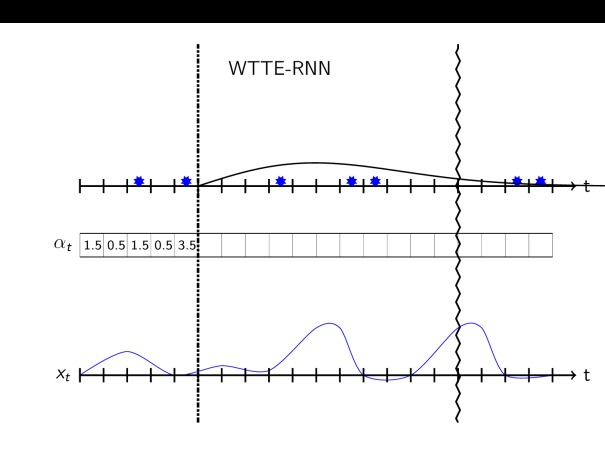
\includegraphics[width=20em]{wtte-4.jpg}}
\fbox{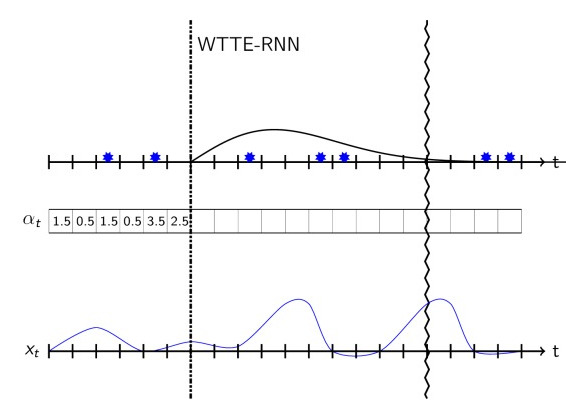
\includegraphics[width=20em]{wtte-5.jpg}}

\fbox{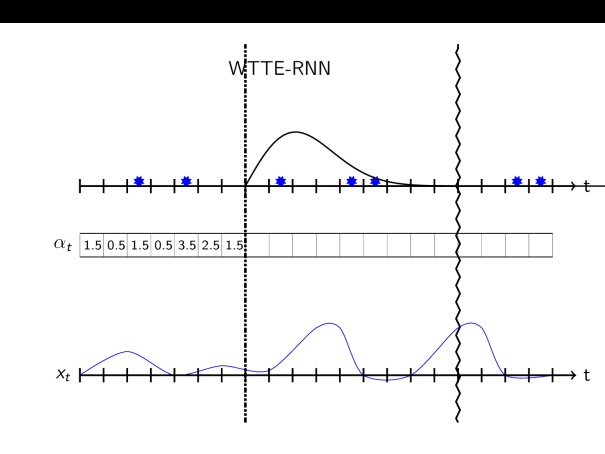
\includegraphics[width=20em]{wtte-6.jpg}}
\fbox{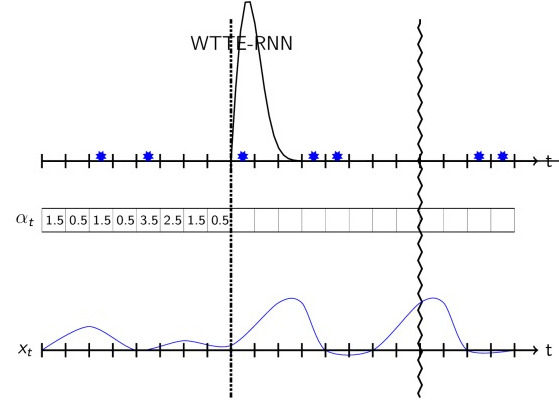
\includegraphics[width=20em]{wtte-7.jpg}}

\fbox{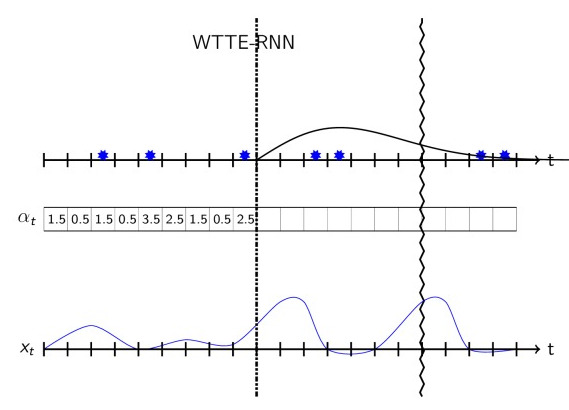
\includegraphics[width=20em]{wtte-8.jpg}}
\fbox{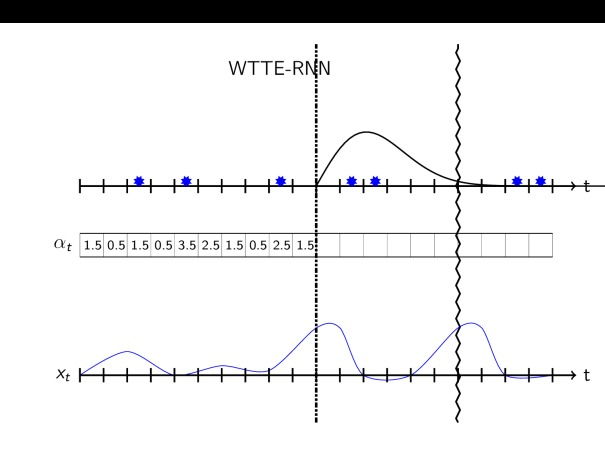
\includegraphics[width=20em]{wtte-9.jpg}}

\fbox{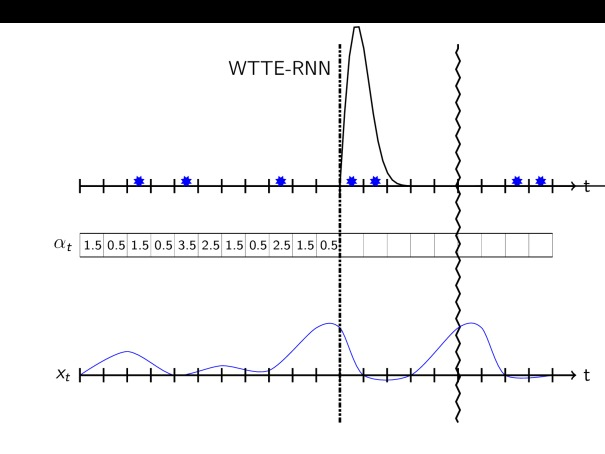
\includegraphics[width=20em]{wtte-10.jpg}}
\fbox{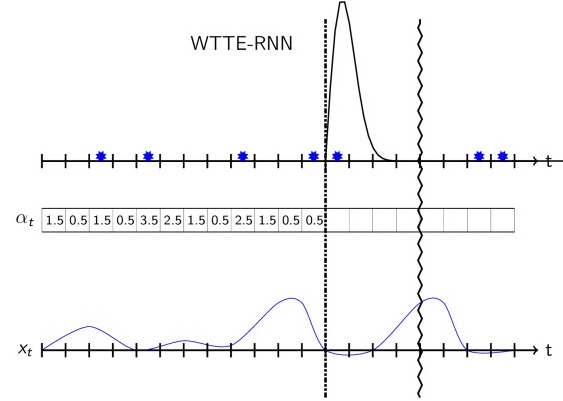
\includegraphics[width=20em]{wtte-11.jpg}}







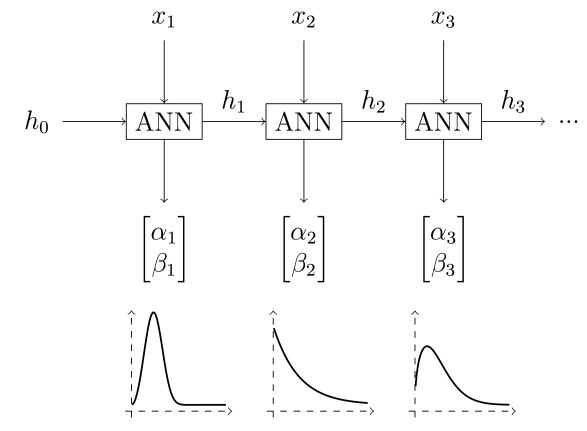
\includegraphics[width=30em]{wtte-rnn.png}




Kaynaklar

[1] Egil, {\em WTTE-RNN - Less hacky churn prediction}, \url{https://ragulpr.github.io/2016/12/22/WTTE-RNN-Hackless-churn-modeling/}

[2] Egil, {\em WTTE-RNN : Weibull Time To Event Recurrent Neural Network}, \url{https://ragulpr.github.io/assets/draft_master_thesis_martinsson_egil_wtte_rnn_2016.pdf}

[3] BPI Challenge 2016, \url{https://www.dropbox.com/s/ou4r5kvypq78hfn/bpi_visit_churn.zip?dl=1}

[4] \url{https://github.com/daynebatten/keras-wtte-rnn}

\end{document}
